\chapter{Lenna -- \emph{Pré-traitement}}
Avant d'essayer de détecter les paragraphes, les lignes ainsi que les caractères dans l'image, et de reconnaître les caractères, il faut "nettoyer" l'image. Dans ce chapitre nous allons décrire différents algorithmes que nous avons implémentés dans ce but.\\

\section{Binarisation}
C'est le premier algorithme que nous avons écrit parce qu'il est simple, essentiel et c'est un bon point de départ pour se familiariser avec la bibliothèque et ses fonctions de base. Nous avons d'abord implémenté la méthode la plus naïve : calculer la moyenne des composantes RGB de chaque pixel pour avoir sa luminosité, et appliquer un seuil. Tout pixel dont la luminosité est en dessous de 127 est considéré comme blanc et les autres comme noir. Evidemment, ce ne fut pas notre algorithme définitif.\\

Nous aurions pu l'améliorer en prenant comme seuil la luminosité moyenne des pixels, cependant cela n'aurais pas été beaucoup mieux. Nous avons plutot décidé de rechercher un meilleur algorithme, et avons décidé que la méthode d'Otsu était la plus adaptée à notre cas. De plus cet algorithme est relativement simple à impémenter. La principe de la méthode d'Otsu est de trouver le seuil idéal pour l'algorithme décrit précedemment. Le seui idéal est défini comme étant celui qui minimise la variance entre les deux classes formées par ce seuil. Il faut donc essayer chaque seuil possible et calculer à chaque fois la variance de chaque classe. Heureusement une petite astuce mathématique nous permet de réduire de façon significative la complexité de cet algorithme en maximisant la variance inter-classe au lieu de minimiser la variance intra-classe.\\

\section{Réduction du bruit}

Nous avons éssayé deux méthodes pour réduire le bruit dans l'image : le flou gaussien et le filtre médian. Nous avons été insatisfait des deux car les lettres étaient moins lisible après le filtre. Pour corriger ça, nous avons réduit le nombre de pixel voisins pris en compte dans le filtre median : pour chaque pixel, nous prenons le pixel median parmi le pixel lui même et ses quatre voisins immédiats.\\

\section{Rotation}
\section{Algorithme de base}

Il est très difficile voir impossible (ou du moins contre-productif) de
détecter des zones de textes, caractères, mots dans une image si cette image
n'est pas droite. C'est pourquoi il est nécessaire, au cours de l'étape de
pré-traitement \emph{pre-processing}, de roter l'image fournie par l'utilisateur
afin qu'elle soit bien adaptée aux étapes de segmentation et d'identification
des caractères. \\

\subsection{Implémentation naive}

Une implémentation naive de la rotation serait l'algorithme suivant. C'est
celui que nous utilisions à la première soutenance mais qui posait quelques
soucis. \\

\begin{itemize}
  \item{Input} \\
    \begin{itemize}
      \item Image de base
      \item Angle de rotation $\theta$
    \end{itemize}
  \item{Output}
    \begin{itemize}
      \item Image rotée
    \end{itemize}
\end{itemize}

\begin{enumerate}

  \item Soit $(w, h)$ les dimensions de l'image de base. Calculer les dimensions
    $(nw, nh)$ de l'image après qu'une rotation d'angle $\theta$ soit appliquée
    sur l'image de base. Visuellement, les dimensions de l'image de base et de
    l'image rotée sont liées par une simple relation trigonométrique.
  \begin{center}
    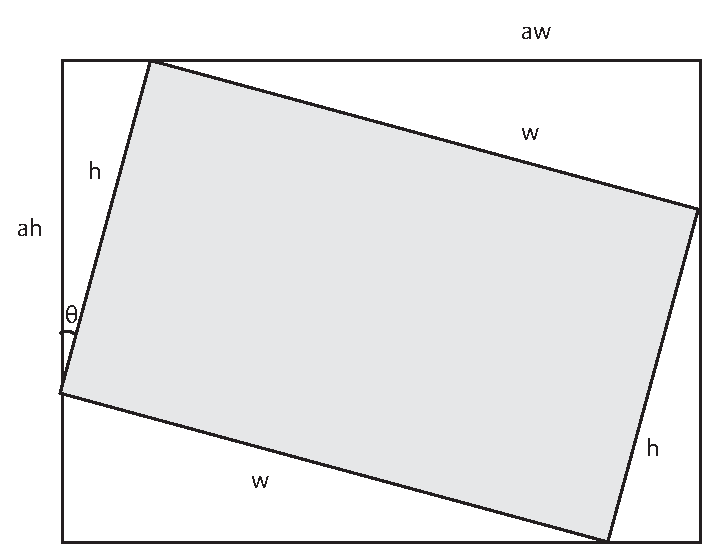
\includegraphics[scale=0.75]{chapters/Pictures/toogy/rotation-new-size.eps}
  \end{center}

  \item Créer une nouvelle image de dimensions $(nw, nh)$ remplie de blanc.

  \item Pour chaque pixel de la nouvelle image, matérialisé par ses coordonnées
    $(x,y)$ dans l'image rotée, calculer ses anciennes coordonnées $(x',y')$
    dans l'image de base. Pour ce faire, on a la relation: \\ 
    $$\begin{pmatrix}x'\\y'\end{pmatrix} =
      \begin{pmatrix}
        \cos\theta & -\sin\theta \\
        \sin\theta & \cos\theta
      \end{pmatrix}
    \begin{pmatrix}
      x \\
      y
    \end{pmatrix}$$

  \item Arrondir ces nouvelles coordonnées et donner aux pixel $(x,y)$ de la
    nouvelle image la couleur du pixel $(x',y')$ de l'image de base. Renvoyer
    l'image.

\end{enumerate}

Cependant, cet algorithme déforme légèrement l'image. Ici, il s'agit de texte et
cette petite déformation réduit énormément sa lisibilité; pour l'homme comme
pour la machine. Il s'agit donc d'être plus intelligent.

\subsection{Interpolation Bilinéaire}

\subsubsection{Interpolation mathématique}

En mathématiques, une interpolation consiste à se servir de données déjà
existante pour approximer des données qui nous manquent. \\

Une interpolation peut se faire de plusieurs façons; plus ou moins précises.
Bien sûr, qui dit plus de précision dit plus de temps de calcul.

\subsubsection{Interpolation bilinéaire appliquée à la rotation}

Ici, il s'agit de se servir des pixels de notre image de base (nos données) pour
déterminer les pixels de notre nouvelle image (les données que nous allons
interpoler). \\

Plusieurs algorithmes d'interpolation existent :
\begin{itemize}
  \item{Nearest-neighbor Interpolation} : le plus simple, il consiste à faire
    la moyenne des composantes $(r,g,b)$ des pixels voisins de notre pixel
    $(x',y')$. C'est le plus rapide.
  \item{Bilinear Interpolation} : un peu plus complexe, il s'agit ici de faire
    deux interpolations linéaires : une entre les deux pixels au dessus de
    $(x',y')$ et une autre entre les deux pixels en dessous de $(x',y')$ (les
    valeurs $x'$ et $y'$ n'étant évidemment pas approximées mais bien située
    entre les entiers de l'arrondi supérieure et de l'arrondi inférieur des
    coordonnées).
    \begin{center}
      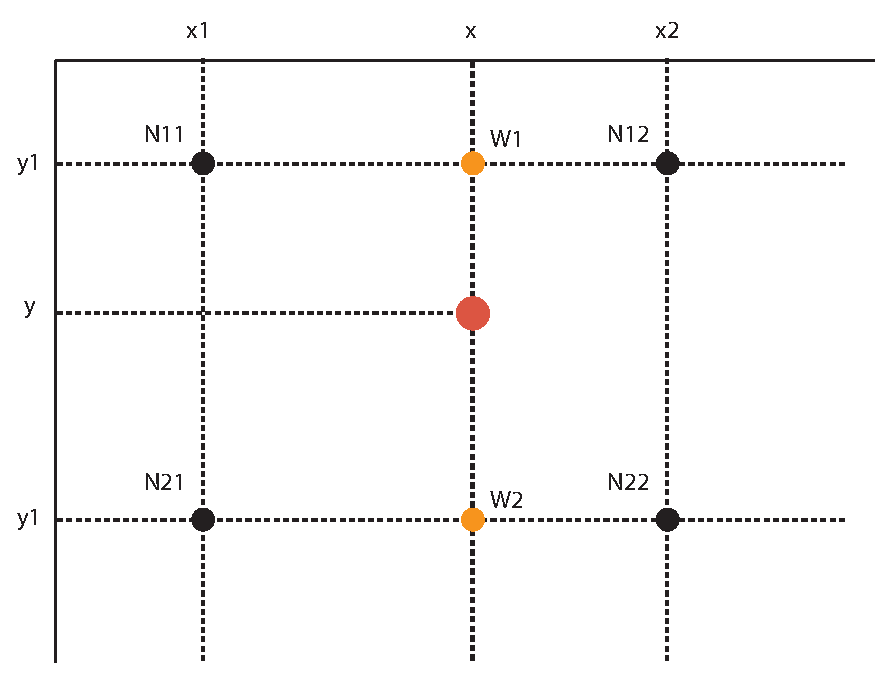
\includegraphics[scale=0.75]{chapters/Pictures/toogy/bilinear.eps}
    \end{center}
    On a alors : \\
    $$W_{1} = \frac{x_{2} - x}{x_{2} - x_{1}} N_{11}
    + \frac{x - x_{1}}{x_{2} - x_{1}} N_{21}$$ \\
    $$\text{et } W_{2} = \frac{x_{2} - x}{x_{2} - x_{1}} N_{12}
    + \frac{x - x_{1}}{x_{2} - x_{1}} N_{22}$$ \\
    Les nouvelles composantes du pixel peuvent alors être calculée via la
    formule \\
    $$R = \frac{y_{2} - y}{y_{2} - y_{1}} W_{1}
    + \frac{y - y_{1}}{y_{2} - y_{1}} W_{2} \text{ \emph{(cas de la
    composante rouge du pixel)}}$$
  \item{Bicubic Interpolation} : plus longue de part son temps de calcul, c'est
    le même principle que pour l'interpolatian bicubique sauf que 8 pixels sont
    étudiés au lieu de 4. Elle donne des résultats plus esthétiques qui ne sont
    pas vraiment utiles dans notre cas.
\end{itemize}

\subsection{Detection de l'angle}
\subsubsection{Transformée de Hough}

La transformée de Hough est une méthode générale pour trouver des lignes et des ellipses dans une image. Elle est souvent utilisée car une fois le principe mathématique compris, elle est simple à implémenter, donne de bons résultats et à une complexité assez faible par rapport, par exemple, à la transformée de Fourier. Nous n'avons besoin que du cas le plus simple de l'algorithme qui consiste à trouver les lignes dans une image binarisée.

La transformée de Hough se base sur une représentation très particulière des droites du plan : plutot que deux les représenter avec les deux paramètres usuels $a$ et $b$ dans l'équation $y = ax + b$, une droite est décrite comme un couple $(r, \theta)$ où $r$ est la distance de la ligne à l'origine et $\theta$ est l'angle de cette distance par rapport à l'abscisse.

  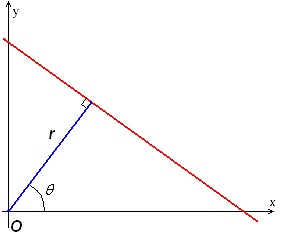
\includegraphics[scale=0.5]{chapters/Pictures/hough1.jpg}\\
En quoi cette représentation est-elle utile? Cela vient du fait que, étant donné un point de coordonnées $(x, y)$ et l'angle $\theta$ de la droite passant par ce point, il est facile d'exprimer la distance $r$ entre la ligne et l'origine. L'équation est la suivante :\\
$r = x\cos\theta + y\sin\theta$\\
Donc pour un point de coordonnées $(x, y)$ on peut tracer le graphe de $r$ en fonction de $\theta$. Il est facile de deviner d'après l'équation que ce graphe sera une sinusoïde. Cette sinusoïde représente l'ensemble des droites passant par ce point. Si nous stockons ce graphe dans un accumulateur, et ajoutons dans cet accumulateur la sinusoïde correspondant à tous les autres points, on obtient un graphe tableau dans lequel la valeur la plus grande représentera les coordonnées de la droite (dans l'espace de Hough) passant par le plus de points possible.

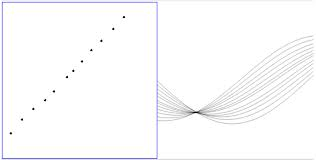
\includegraphics[scale=0.7]{chapters/Pictures/hough2.jpg}\\
\subsubsection{Plus de pré-traitement}

Il y'a encore un problème à régler avant de pouvoir appliquer la transformée de Hough à notre image scannée : Une ligne de texte n'apparait pas comme une ligne droite. Nous avons essayé d'appliquer directement à une image binarisée, mais la plupart du temps il trouvait ou bien la diagonale de l'image, ou bien une reliure particulièrement visible. Après quelques recherches, nous avons trouvé une solution : on détecte tout d'abord les blocs de pixels noirs connexes, qui ne sont pas toujours mais très souvent des caractères, et on les remplaces par leur point centrale. L'utilité est triple : rendre plus apparentes (du point de vue de la transformée de Hough) les lignes de texte, réduire considérablement la complexité de l'algorithme et reduire l'importance des gros blocs de pixels comme les tâches ou les reliures. Voici un exemple de sortie :

\begin{figure}[h!]\
    \centering
    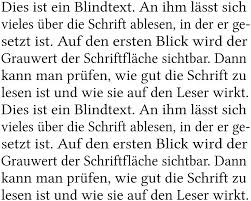
\includegraphics[scale=1]{chapters/Pictures/hough3.jpg}
    \caption{input image}
\end{figure}
\begin{figure}[h!]\
    \centering
    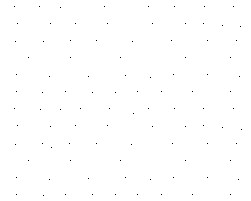
\includegraphics[scale=1]{chapters/Pictures/hough4.jpg}
    \caption{center of each block}
\end{figure}
\begin{figure}[h!]\
    \centering
    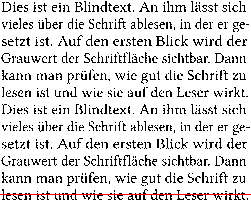
\includegraphics[scale=1]{chapters/Pictures/hough5.png}
    \caption{line found by the Hough transform}
\end{figure}
